\section{\Large PROBLEM SET 8}
\subsection{PROBLEM 1}
\textit{The time update should be complete and verified at this stage. We need to include the incoming measurements. Search in literature or derive, define, and code a sensitivity matrix \textbf{H} which provides your state at step k+1 from your measurement vector at step k+1 (i.e., at the same current time, propagation has already been done).}

The following equations define the sensitivity matrix $\mathbf{H_k}$ for the case where there are $n$ unit direction vector measurements (sun sensors, star trackers, etc.), and a 3-axis rate gyroscope measurement.

\begin{align*}
    \mathbf{H} = \frac{\delta \mathbf{h}}{\delta \mathbf{x}} =
    \begin{bmatrix}
        [\mathbf{h_1} \times] & \mathbf{0}_{3 \times 3} \\
        [\mathbf{h_2} \times] & \mathbf{0}_{3 \times 3} \\
        ... & ... \\
        [\mathbf{h_n} \times] & \mathbf{0}_{3 \times 3} \\
        \mathbf{0}_{3 \times 3} & \mathbf{I}_{3 \times 3} \\
    \end{bmatrix}
\end{align*}

In the equation above, $[\mathbf{h_i} \times]$ refers to the cross-product matrix for the measurement vector $\mathbf{h_i}$.

\subsection{PROBLEM 2}
\textit{Define and code your constant measurement error covariance matrix \textbf{R} which quantifies the uncertainty of your measurements. This can be picked as diagonal matrix with diagonal elements representing the variance of each parameter $\sigma^{2}_{m}$. Hint: If your instrument is well characterized you can use $\sigma_{m}$ applied in your simulation to generate the measurements from your ground-truth.}

For the sensors used in our measurements, $\mathbf{R}$ is defined as a diagonal matrix of the sensor variances discussed in Problem Set 7, Problem 1 (where the sensor errors are based on the variance of the white noise in each case).

\begin{align*}
    \mathbf{R} = 
    \begin{bmatrix}
        diag(\sigma_{star tracker}^2) & \mathbf{0} & \mathbf{0} \\
        \mathbf{0} & diag(\sigma_{sun sensor}^2) & \mathbf{0} \\
        \mathbf{0} & \mathbf{0} & diag(\sigma_{gyroscopes}^2)\\
    \end{bmatrix}
\end{align*}

\subsection{PROBLEM 3}
\textit{Compute your modelled measurement vector at step k+1 from your state at step k+1. 
This transformation can be rigorous (non-linear, EKF) or approximate (linear, KF).}

We continue with our modeling for an MEKF system. The modeled measurement vector at step k+1 was found by plugging the estimated state at step k+1 into the previously developed measurement model, without measurement noise.

Our modeled measurement uses simulated unit vectors describing directions for a star tracker and sun sensor. We also provide angular velocity data from simulation with noise to simulate a rate gyro. Our functions for the star tracker and sun sensor in the modeled measurements are shown below.

\lstinputlisting{src/starTracker.m}

\lstinputlisting{src/sunSensor.m}

\subsection{PROBLEM 4}
\textit{Compute your pre-fit residuals \textit{z} by differencing modeled and actual measurement vector at k+1.}

The pre-fit residuals were calculated as the difference of the output (raw measurements with noise) and the modeled measurements based on our the measurement model and state prior to the measurement update.

\subsection{PROBLEM 5}
\textit{The measurement update of the EKF needs \textbf{H}, \textbf{P}, \textbf{R}, and \textbf{z} to compute the Kalman gain \textbf{K}, the new estimated state and its associated covariance matrix.}

The following equations are used in the measurement step calculation.

\begin{align*}
    \mathbf{x_{k+1 | k+1}} = \mathbf{x_{k+1 | k}} + \mathbf{K_k}
    (\mathbf{y_k} - \mathbf{z_k}) \\
    \mathbf{P_{k+1 | k+1}} = \mathbf{P_{k+1 | k}} - 
    \mathbf{K_k} \mathbf{H_k} \mathbf{P_{k+1 | k}} \\
    \mathbf{K_k} = \mathbf{P_{k+1 | k}} \mathbf{H_k}^T [\mathbf{H_k} \mathbf{P_{k+1 | k}} \mathbf{H_k}^T + \mathbf{R_k}]^{-1}
\end{align*}

We implement the measurement update in code with the following function. This MATLAB function is used as part of our Simulink model.

\lstinputlisting{src/measurementUpdate.m}

Our entire MEKF is modeled in Simulink, as shown in the diagram below.

\begin{figure}[H]
\centering
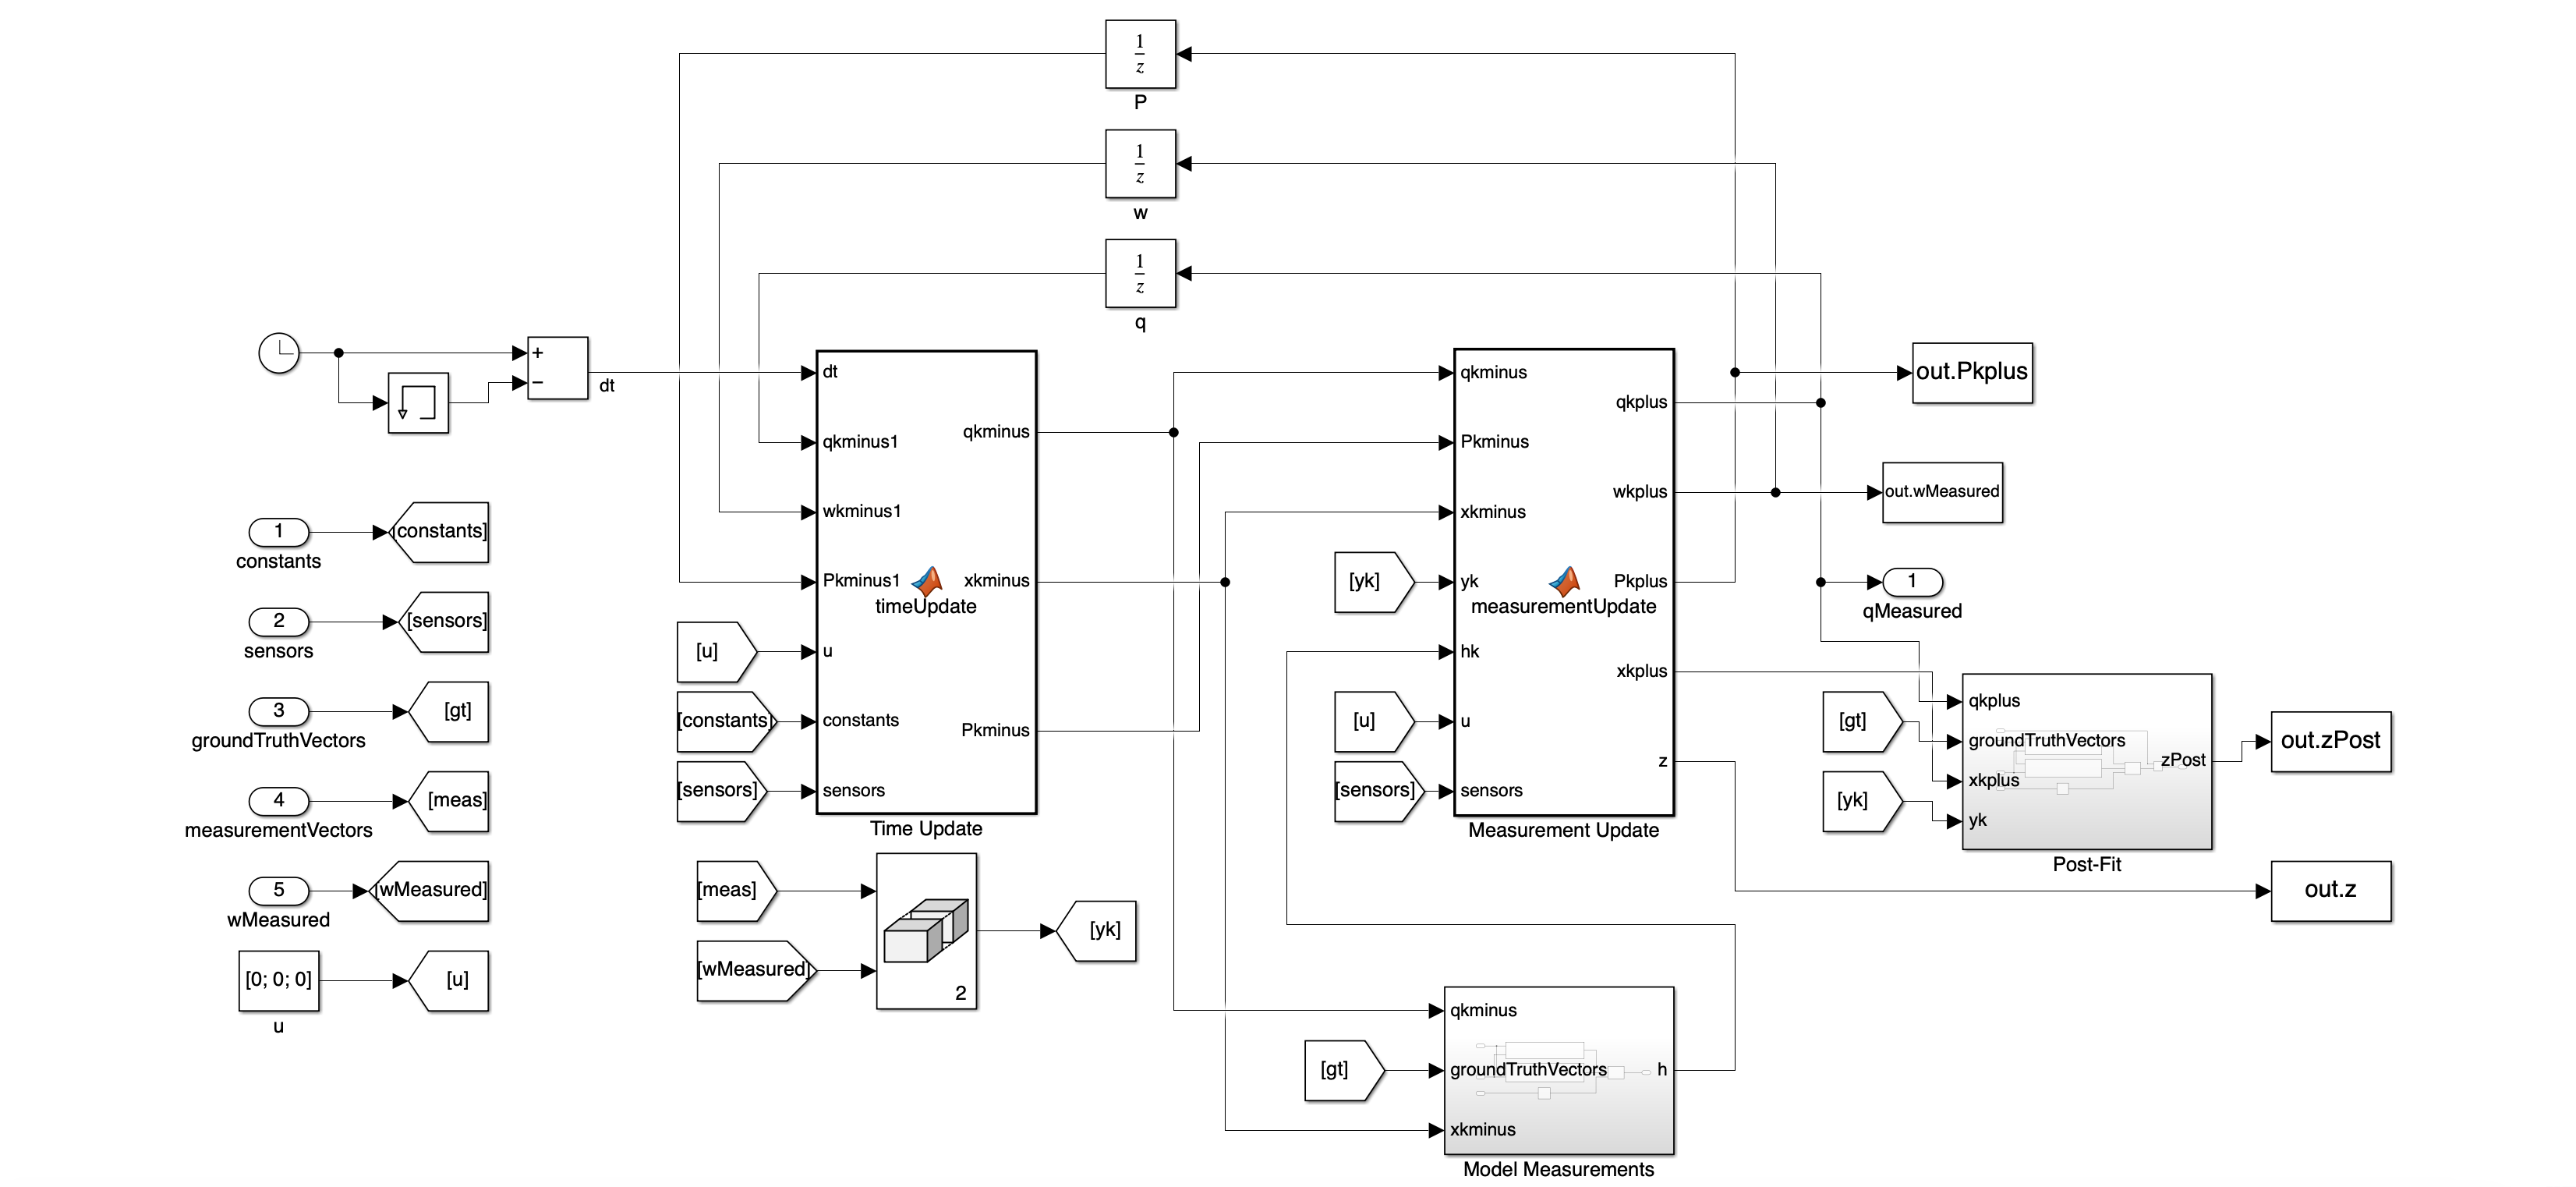
\includegraphics[scale=0.27]{Images/ps8_problem5_simulink.png}
\caption{Simulink model of MEKF}
\label{fig:ps8_problem5_simulink}
\end{figure}

\newpage
\subsection{PROBLEM 6}
\textit{Compute your post-fit residuals z by differencing modelled and actual measurement vector at k+1 using your new state. These should be smaller than the pre-fit residuals and should capture the standard deviation of your measurements at steady state.}

The post-fit residuals z are found by taking the updated state from the measurement update step and computing a modeled measurement using our measurement model again. Figures \ref{fig:ps8_problem7_res_units} and \ref{fig:ps8_problem7_res_gyro} show the plots of the pre- and post-fit residuals.

\subsection{PROBLEM 7}
\textit{Produce plots showing true attitude estimation errors (estimate vs truth with statistics at steady state), formal or estimated attitude estimation errors (covariance from filter), pre- and post-fit residuals (with statistics at steady state), etc. Discuss the results, do they meet expectations? Is the true estimation error well described by the formal covariance? Are the measurements residuals consistent with the applied measurement errors? Hint: show estimation errors, do not overlap state estimate with reference truth.}

Below are the error and residual plots. Figure \ref{fig:ps8_problem7_error} shows the attitude estimate errors with the MEKF method. As expected, the errors are very small compared to the attitude determination methods used in the previous section.

Figure \ref{fig:ps8_problem7_cov} shows the estimated attitude determination errors based on the covariance of the filter. Comparing this with Figure \ref{fig:ps8_problem7_error}, it seems that this method may under-report the error and is not necessarily the most accurate representation of error.

\begin{figure}[H]
\centering
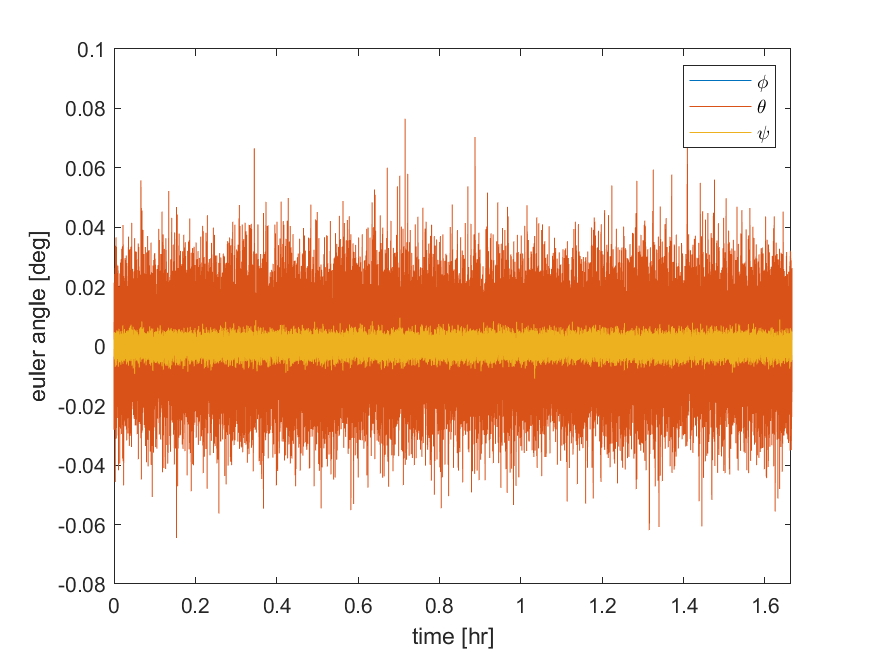
\includegraphics[scale=0.8]{Images/ps8_problem7_error.png}
\caption{Errors between MEKF measurements and ground truth}
\label{fig:ps8_problem7_error}
\end{figure}

\begin{figure}[H]
\centering
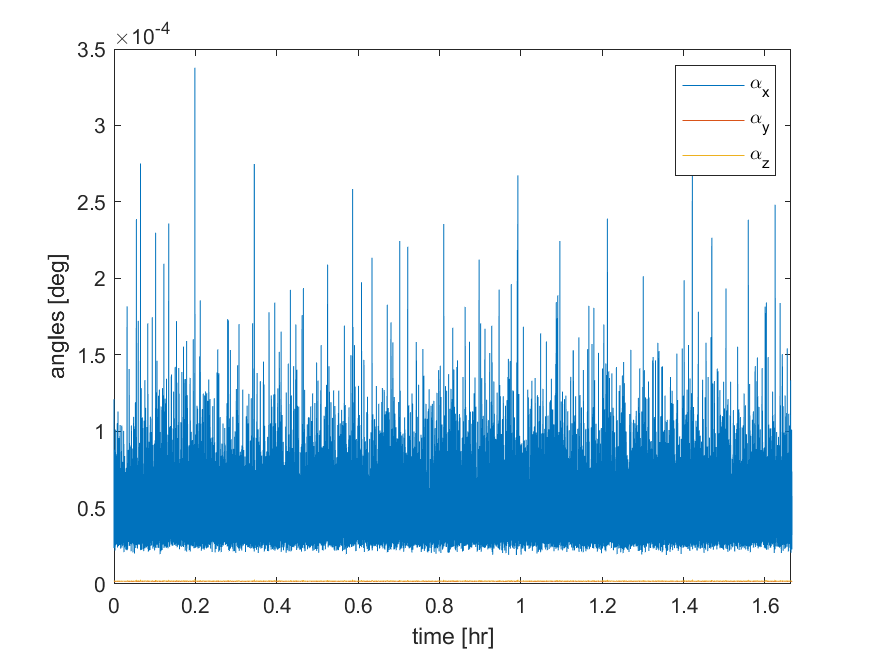
\includegraphics[scale=0.8]{Images/ps8_problem7_cov.png}
\caption{Estimated attitude estimation errors from covariance (small angles)}
\label{fig:ps8_problem7_cov}
\end{figure}

Figures \ref{fig:ps8_problem7_res_units} and \ref{fig:ps8_problem7_res_gyro} below show the difference in the norms of the pre-fit and post-fit residuals. As expected, the post-fit residuals are slightly smaller than the pre-fit residuals. However, the difference between pre-fit and post-fit sensor noise is much better for the gyroscope measurements than the unit direction vector measurements.

\begin{figure}[H]
\centering
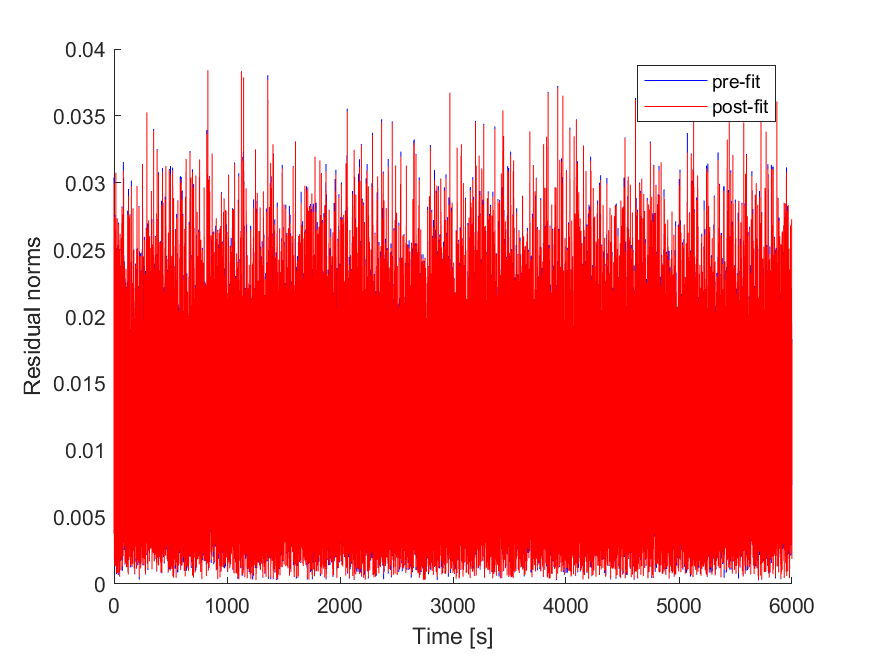
\includegraphics[scale=0.8]{Images/ps8_problem7_res_units.png}
\caption{Norm of pre-fit and post-fit direction-vector residuals}
\label{fig:ps8_problem7_res_units}
\end{figure}

\begin{figure}[H]
\centering
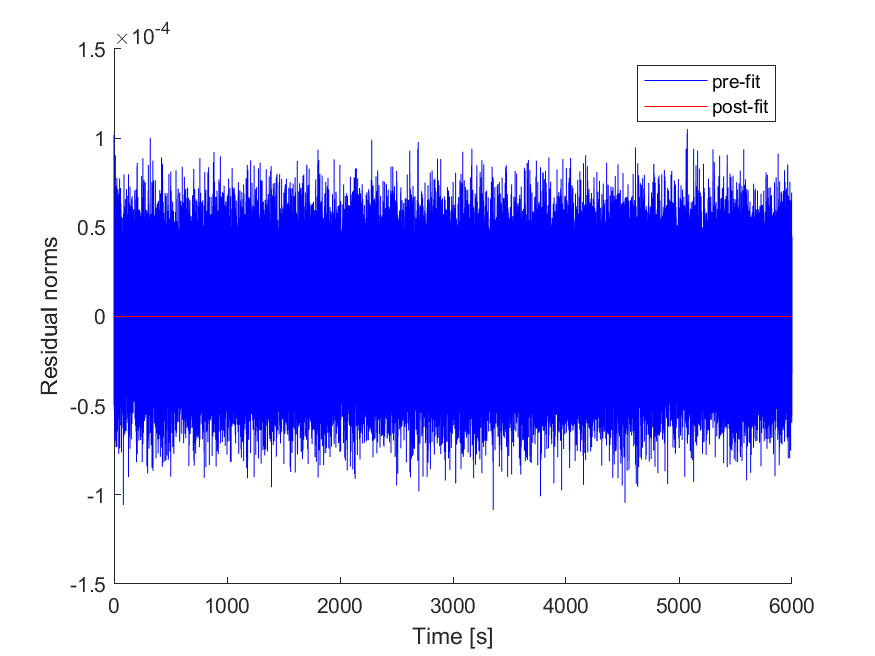
\includegraphics[scale=0.8]{Images/ps8_problem7_res_gyro.png}
\caption{Pre-fit and post-fit gyroscope residuals}
\label{fig:ps8_problem7_res_gyro}
\end{figure}

Investigating the measurement model, noise model, and sensitivity matrix for the unit vector-based measurements, we may be able to improve the performance shown in Figure \ref{fig:ps8_problem7_res_units}. This is an area for potential future work, as well as the topics discussed in the following section.

\subsection{PROBLEM 8}
\textit{Start thinking/planning possible upgrades for the final project deliverable. Upgrades can go in several directions tailored to your project needs. For example, define different modes for attitude estimation using different sensors and algorithms based on your concept of operations. What would it take to implement a UKF instead of an EKF? Can you improve your dynamics and measurement models? Can you use measurements that are more representative of what your sensors are going to actually provide you? Hint: you should not panic if your Kalman filter is not working, you can always address the rest of the problem sets bypassing the Kalman filter. Do not give up though!}

One possible upgrade for the final project could be to include biases in the EKF state such that we can track drift. Strictly adhering to the assumptions of the Kalman filter, we should have unbiased measurements in our system, and we should be correcting the value of the measurements which is passed into the filter using the bias or drift which we track. However, this would require modeling the dynamics of the drift in order to simulate properly.

We also have an opportunity to model the magnetic field–we have already implemented a fourth-order magnetic field model, but additional refinements and fixes could improve this model and make it usable for attitude determination in conjunction with a magnetometer. We can also take advantage of the magnetic field for actuation via magnetorquers.

An interesting topic to study is whether our system is able to accurately predict the attitude of the satellite within the pointing requirements necessary for NISAR to successfully collect science data. These requirements are available in literature for comparison, and we can also examine the effect of this on the image swath captured by the SAR sensor suite.

Finally, a substantial project could be to model the intricacies of the star tracker, such as implementing algorithms for matching stars to a star catalog (as well as incorporating the star catalog itself). This would require modeling the field of view of each star tracker and stars in the celestial sphere.